% vim: set tw=78 aw:
\documentclass{beamer}

\usepackage[utf8x]{inputenc} % diacritice
\usepackage[romanian]{babel}
\usepackage{color}			 % highlight
\usepackage{alltt}			 % highlight
\usepackage{code/highlight}	 % highlight
\usepackage{hyperref}        % folositi \url{http://...}
                             % sau \href{http://...}{Nume Link}
\mode<presentation>
{ \usetheme{Rochester} }		% TODO: settle this

% Titlul nu foloseşte Unicode pentru că e o problemă căreia nu i-am dat de
% cap.
\title[Merger si comparator de fișiere]{Merger si comparator de fisiere}
\subtitle{CDL - Proiecte}
\institute{ROSEdu}
\author{Lucian Adrian Grijincu \\ \texttt{lucian.grijincu@rosedu.org}}

\begin{document}

% Slide-urile cu mai multe părţi sunt marcate cu textul (cont.)
\setbeamertemplate{frametitle continuation}[from second]
% Arătăm numărul frame-ului
\setbeamertemplate{footline}[frame number]

\frame{\titlepage}

\frame{\tableofcontents}






\section{De ce?}
\frame{\tableofcontents[currentsection]}

\begin{frame}{De ce?}
  \begin{itemize}
  \item țineți minte cum arătau fișierele patch?
  \end{itemize}
\end{frame}

\begin{frame}{Urât!}
  \input{code/diff_u}
\end{frame}

\begin{frame}{De ce?}
  \begin{itemize}[<+->]
  \item la dimensiuni mari outputul în format diff (fișier patch) este dificil de urmărit.
  \item nu este flexibil: 
    \begin{itemize}
    \item dacă vrem să modificăm vre-un parametru (de ex. numărul de linii de context) trebuie executată o nouă comandă \texttt{diff}
    \end{itemize}
  \item lipsa \textit{syntax-highliting} atunci când se revizuiesc patchurile
  \item modificarea unui fișier patch este dificilă (trebuie modificate metadatele
  \end{itemize}
\end{frame}













\section{MELD}
\frame{\tableofcontents[currentsection]}

\begin{frame}{Un alt mod de a vizualiza diferențele?}
  \begin{itemize}
  \item nu ar fi mai ușor de urmărit dacă am avea fișierele de comparat unul lângă altul?
    \pause
    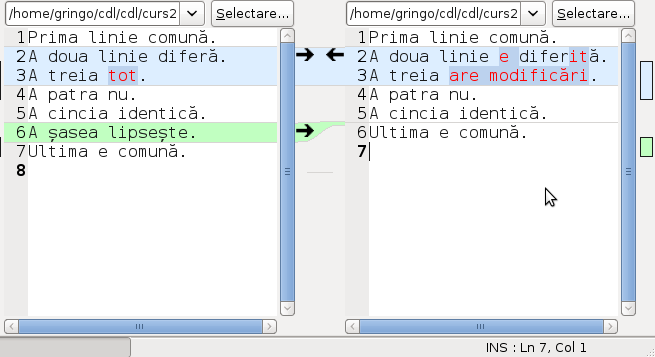
\includegraphics[height=5cm]{code/screenshot-meld.png}%
  \end{itemize}
\end{frame}

\begin{frame}{Un alt mod de a vizualiza diferențele : MELD}
  \begin{itemize}[<+->]
  \item captura de ecran anterioară este din MELD
    \begin{itemize}
      \item \texttt{sudo apt-get install meld}
    \end{itemize}
  \item meld are limitări:
    \begin{itemize}
      \item dacă algoritmul care detectează zonele similare și cele diferite nu 
        funcționează corect acestea nu pot fi specificate de utilizator
      \item nu permite vizualizarea diferențelor între resurse non-text
        \begin{itemize}
        \item imagini
        \item metadata imagini (EXIF data)
        \item fișiere binare
          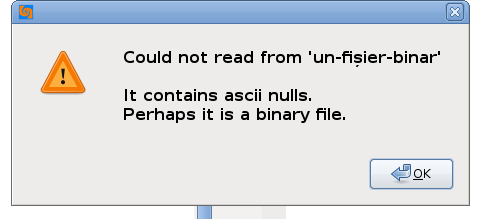
\includegraphics[height=2cm]{code/screenshot-meld-binary-error.png}
        \end{itemize}
    \end{itemize}
  \end{itemize}
\end{frame}











\section{Beyond Compare}
\frame{\tableofcontents[currentsection]}

\begin{frame}{Un exemplu comercial : Beyond Compare}
  \begin{itemize}
    \item suport pentru comparare imagini (pixel cu pixel)
      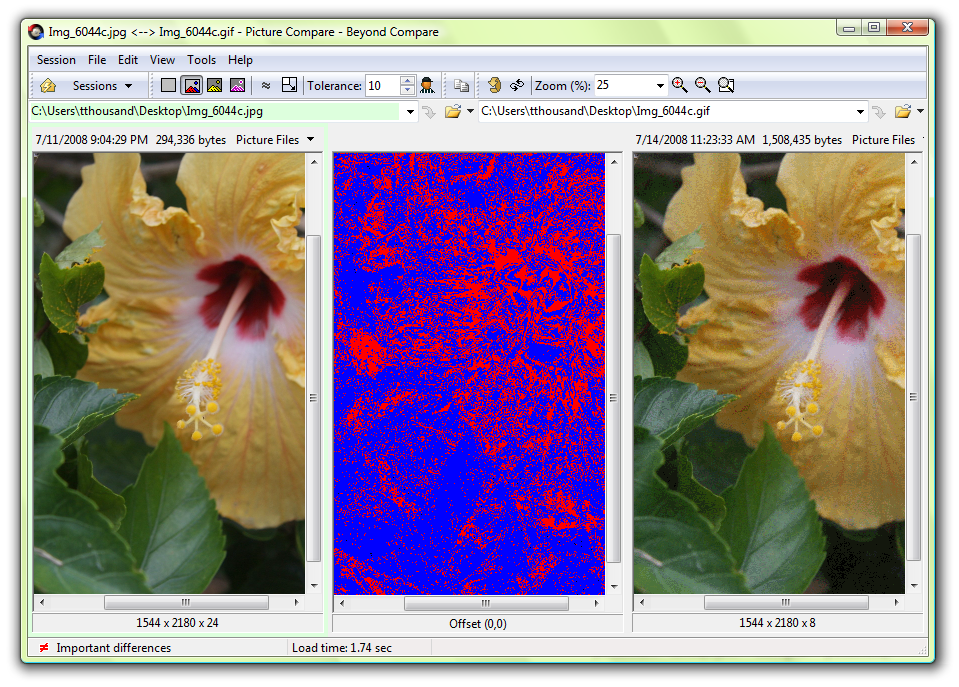
\includegraphics[height=5cm]{code/bc-imagini.png}
  \end{itemize}
\end{frame}

\begin{frame}{Un exemplu comercial : Beyond Compare}
  \begin{itemize}      
      \item comparare fișiere binare
      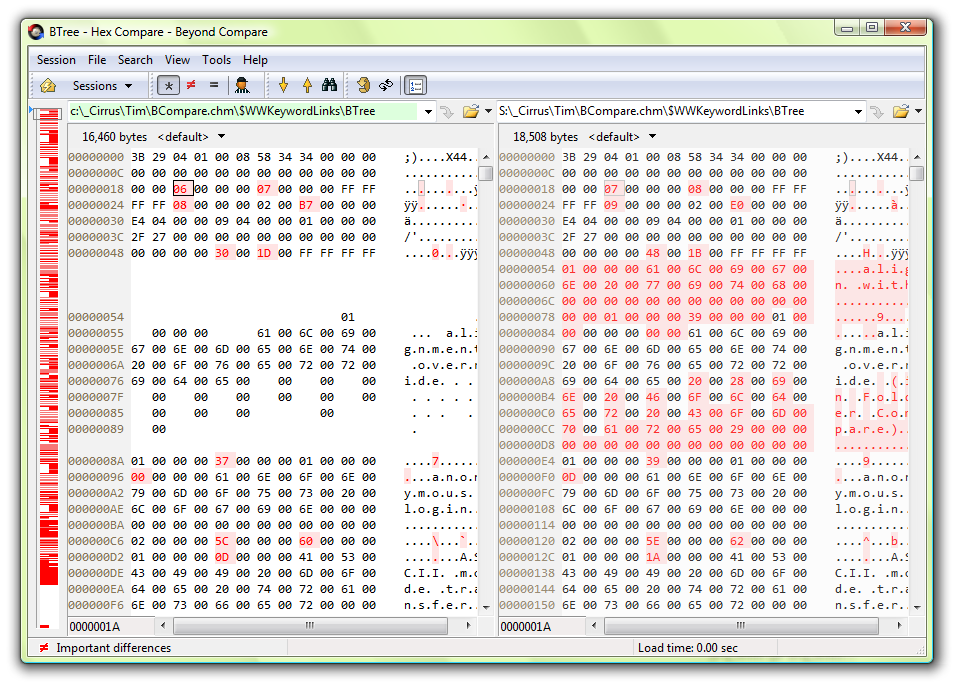
\includegraphics[height=5cm]{code/bc-hex.png}
  \end{itemize}
\end{frame}

\begin{frame}{Un exemplu comercial : Beyond Compare}
  \begin{itemize}      
      \item comparare fișiere CVS (comma separated values)
      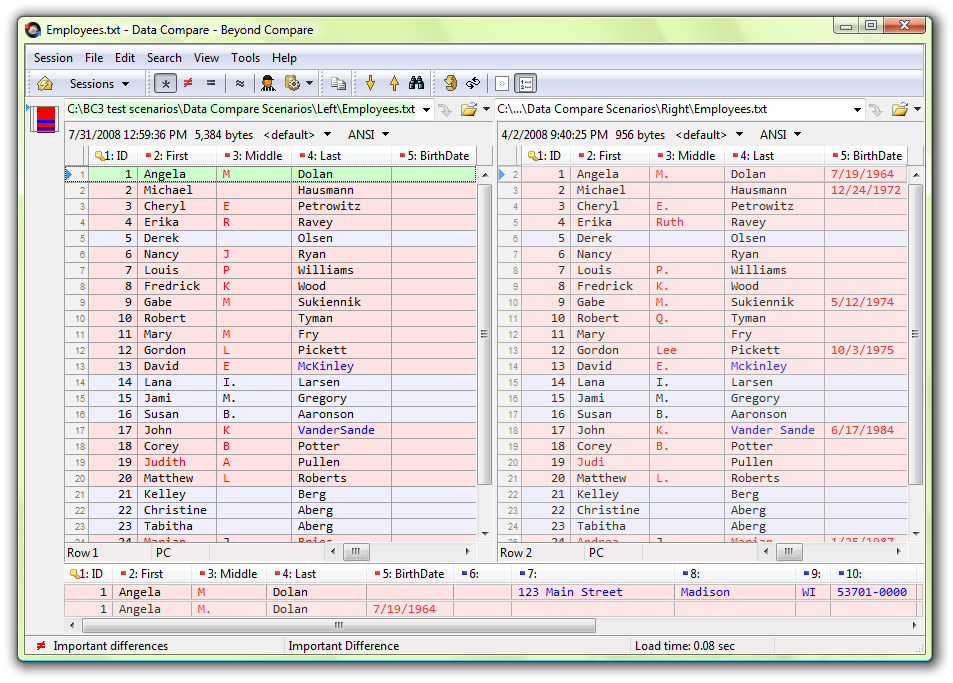
\includegraphics[height=5cm]{code/bc-cvs.png}
  \end{itemize}
\end{frame}

\begin{frame}{Un exemplu comercial : Beyond Compare}
  \begin{itemize}      
      \item comparare fișiere text
        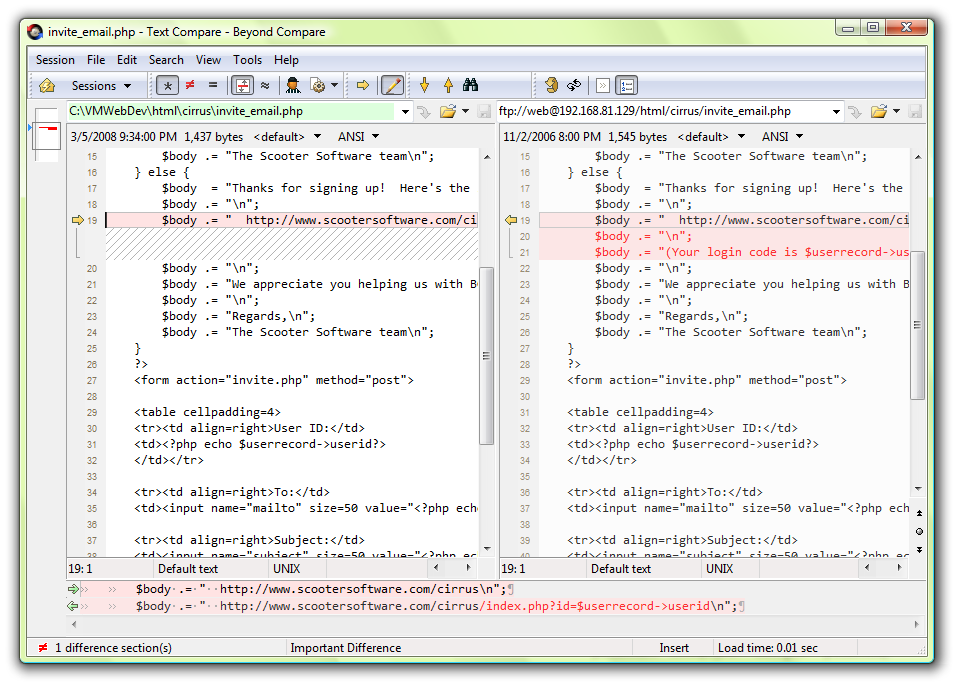
\includegraphics[height=5cm]{code/bc-text.png}
  \end{itemize}
\end{frame}









\section{Proiect CDL}
\frame{\tableofcontents[currentsection]}

\begin{frame}{Ce facem?}
  \begin{itemize}[<+->]
  \item mai multe tipuri de fișiere suportate
  \item eliminarea limitărilor pe care le are \texttt{meld}
  \item ???
  \item profit!
  \end{itemize}
\end{frame}


\end{document}
